  \begin{figure}
    \centering

    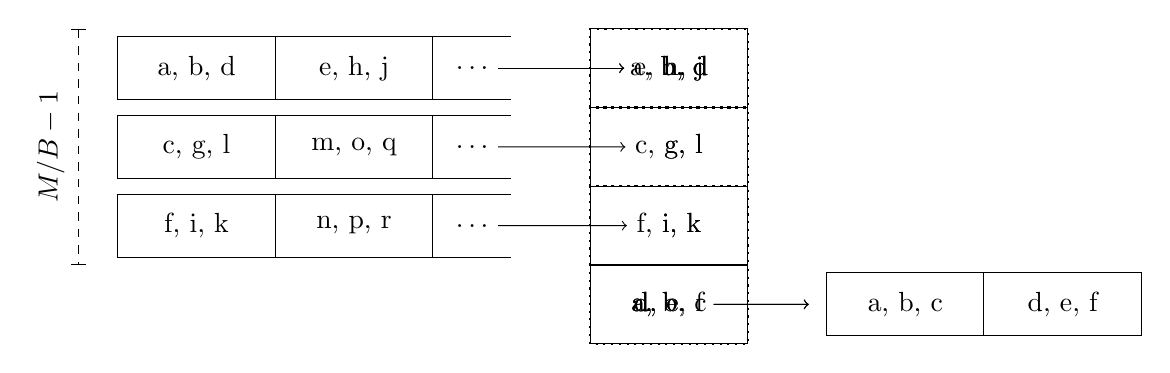
\begin{tikzpicture}
      % Input Blocks
      \draw[] (0,0.1)  rectangle ++(2,0.8) node[pos=.5] {a, b, d};
      \draw[] (2,0.1)  rectangle ++(2,0.8) node[pos=.5] {e, h, j};
      \draw[-] (4,0.9) -- ++(1,0);
      \node[] at (4.5,0.5) (i1) {$\dots$};
      \draw[-] (4,0.1) -- ++(1,0);

      \draw[] (0,-0.9) rectangle ++(2,0.8) node[pos=.5] {c, g, l};
      \draw[] (2,-0.9) rectangle ++(2,0.8) node[pos=.5] {m, o, q};
      \draw[-] (4,-0.1) -- ++(1,0);
      \node[] at (4.5,-0.5) (i2) {$\dots$};
      \draw[-] (4,-0.9) -- ++(1,0);

      \draw[] (0,-1.9) rectangle ++(2,0.8) node[pos=.5] (i3b1) {f, i, k};
      \draw[] (2,-1.9) rectangle ++(2,0.8) node[pos=.5] (i3b2) {n, p, r};
      \draw[-] (4,-1.1) -- ++(1,0);
      \node[] at (4.5,-1.5) (i3) {$\dots$};
      \draw[-] (4,-1.9) -- ++(1,0);

      % Input Blocks Size
      \draw [black, dashed, |-|] (-0.5,1) -- node[pos=.5, rotate=90, yshift=10] {$M/B-1$} (-0.5,-2);

      % Memory

      % - I1
      \draw[dotted, thick] (6,0)  rectangle ++(2,1) node[pos=.5] (M1) {};

      \onslide<2-3> {
        \draw[] (6,0)  rectangle ++(2,1) node[pos=.5] (M1) {a, b, d};
      }
      \onslide<4> {
        \draw[] (6,0)  rectangle ++(2,1) node[pos=.5] (M1) {\phantom{a, }b, d};
      }
      \onslide<5-8> {
        \draw[] (6,0)  rectangle ++(2,1) node[pos=.5] (M1) {\phantom{a, b, }d};
      }

      \onslide<10-11> {
        \draw[] (6,0)  rectangle ++(2,1) node[pos=.5] (M1) {e, h, j};
      }
      \onslide<12-> {
        \draw[] (6,0)  rectangle ++(2,1) node[pos=.5] (M1) {\phantom{e, }h, j};
      }

      % - I2
      \draw[dotted, thick] (6,-1)  rectangle ++(2,1) node[pos=.5] (M2) {};

      \onslide<2-5>{
        \draw[] (6,-1)  rectangle ++(2,1) node[pos=.5] (M2) {c, g, l};
      }
      \onslide<6->{
        \draw[] (6,-1)  rectangle ++(2,1) node[pos=.5] (M2) {\phantom{c, }g, l};
      }

      % - I3
      \draw[dotted, thick] (6,-2)  rectangle ++(2,1) node[pos=.5] (M3) {};

      \onslide<2-12>{
        \draw[] (6,-2)  rectangle ++(2,1) node[pos=.5] (M3) {f, i, k};
      }
      \onslide<13->{
        \draw[] (6,-2)  rectangle ++(2,1) node[pos=.5] (M3) {\phantom{f, }i, k};
      }

      % - O
      \draw[dotted, thick] (6,-3)  rectangle ++(2,1) node[pos=.5] (M4) {};

      \onslide<4> {
        \draw[] (6,-3)  rectangle ++(2,1) node[pos=.5] (M4) {a\phantom{, b, c}};
      }
      \onslide<5> {
        \draw[] (6,-3)  rectangle ++(2,1) node[pos=.5] (M4) {a, b\phantom{, c}};
      }
      \onslide<6> {
        \draw[] (6,-3)  rectangle ++(2,1) node[pos=.5] (M4) {a, b, c};
      }

      \onslide<9-11> {
        \draw[] (6,-3)  rectangle ++(2,1) node[pos=.5] (M4) {d\phantom{, e, f}};
      }
      \onslide<12> {
        \draw[] (6,-3)  rectangle ++(2,1) node[pos=.5] (M4) {d, e\phantom{, f}};
      }
      \onslide<13> {
        \draw[] (6,-3)  rectangle ++(2,1) node[pos=.5] (M4) {d, e, f};
      }

      % Output blocks
      \node[] at (8.9,-2.5) (o) {};
      \onslide<7-> {
        \draw[] (9,-2.9)   rectangle ++(2,0.8) node[pos=.5] (ob1) {a, b, c};
      }
      \onslide<14-> {
        \draw[] (11,-2.9) rectangle ++(2,0.8) node[pos=.5] (ob2) {d, e, f};
      }

      % Arrows
      \onslide<2> {
        \draw[->]
          (i1) edge (M1)
          (i2) edge (M2)
          (i3) edge (M3)
        ;
      }
      \onslide<7> {
        \draw[->] (M4) edge (o);
      }
      \onslide<10> {
        \draw[->] (i1) edge (M1);
      }
      \onslide<14> {
        \draw[->] (M4) edge (o);
      }
    \end{tikzpicture}
  \end{figure}
